\documentclass[12pt]{article}

\usepackage{fontspec}
\usepackage{amsmath, amssymb, amsfonts}
\usepackage{graphicx}
\usepackage{hyperref}
\usepackage{color}
\usepackage{geometry}
\geometry{a4paper}
\usepackage{pgfplots}

\begin{document}
	\begin{minipage}[t]{.5\textwidth}
		{\large Prénom :\\
		Nom :}
	\end{minipage}%
	\begin{minipage}[t]{.5\textwidth}
		\begin{flushright}
			{\Large /10}
		\end{flushright}
	\end{minipage}

	\vspace{3em}
	\begin{center}
			{\Large Interrogation : les équations vectorielles de droites et de plans}\\
			{\large 6e Générale}\\
			$1^{\text{er}}$ décembre 2023
	\end{center}
	
	\vspace{3em}
	
	\textbf{Consignes :} Tu peux écrire sur cette feuille ou sur une feuille à part, n'oublie pas de bien écrire tes prénom et nom sur toutes les feuilles que tu utilises. Les machines à calculer sont autorisées. Pose des questions si tu en as besoin. Bon courage !
	
	\vspace{2em}
	
	\begin{enumerate}
		\item 
			\begin{minipage}[t]{.9\textwidth}
				Donne la formule de l'équation vectorielle d'un \textbf{plan} en définissant tous les éléments qui y apparaissent.
			\end{minipage}%
			\begin{minipage}{.1\textwidth}
				\begin{flushright}
					{\large /2}
				\end{flushright}
			\end{minipage}
			\vspace{3em}
			
		\item 
			\begin{minipage}[t]{.9\textwidth}
				Donne l'équation vectorielles des figures suivantes :
				\begin{enumerate}
					\item La droite $D$ de vecteur directeur $\left(1; -2; 3 \right)$ et passant par le point $\left(1; 0; 1\right)$.
					\item Le plan $P$ de vecteurs directeurs $\left(1; 1; 3\right)$ et $\left(-2; 1; 1\right)$ et passant par le point $\left(0; 1; 0\right)$.
				\end{enumerate}
			\end{minipage}%
			\begin{minipage}{.1\textwidth}
				\begin{flushright}
					{\large /2}
				\end{flushright}
			\end{minipage}
			\vspace{3em}
			
		\item 
			\begin{minipage}[t]{.9\textwidth}
				Soit le plan $P$ d'équation $P \equiv \vec{x} = k_1 \cdot \left(0; 1; 2\right) + k_2 \cdot\left(3; 2; -1\right) + \left(1; 1; 1\right), ~(k_1, k_2 \in \mathbb{R})$. Donne l'équation d'un plan $R$ \textbf{orthogonal} à $P$.
			\end{minipage}%
			\begin{minipage}{.1\textwidth}
				\begin{flushright}
					{\large /2}
				\end{flushright}
			\end{minipage}
			\vspace{3em}
			
		\item 
			\begin{minipage}[t]{.9\textwidth}
				Donne l'équation de la droite qui passe par les points $A$ et $B$ représenté dans le repère orthonormé ci-dessous :
				\begin{center}
					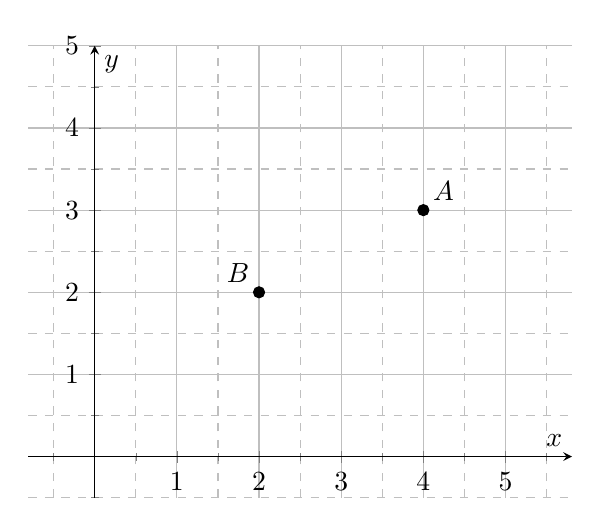
\begin{tikzpicture}
						\begin{axis}[
							width=.7\linewidth,
							axis lines=center,
							xlabel={$x$},
							ylabel={$y$},
							xmin=0, xmax=5,
							ymin=-0.5, ymax=5,
							axis equal,
							grid=both,
							minor tick num=1,
							minor grid style={dashed}
							]
							
							\addplot[only marks, mark=*] coordinates {(4, 3)} node[above right] {$A$};
							\addplot[only marks, mark=*] coordinates {(2, 2)} node[above left] {$B$};
							
						\end{axis}
					\end{tikzpicture}
				\end{center}
			\end{minipage}%
			\begin{minipage}{.1\textwidth}
				\begin{flushright}
					{\large /2}
				\end{flushright}
			\end{minipage}
			\vspace{3em}
			
		\item 
			\begin{minipage}[t]{.9\textwidth}
				Soit les figures suivantes :
				\begin{itemize}
					\item Le plan $P$ d'équation $P \equiv \vec{x} = k_1 \cdot \left(1; 1; 1\right) + k_2 \cdot\left(0; 1; 2\right) + \left(0; 0; 1\right), ~(k_1, k_2 \in \mathbb{R})$.
					\item La droite $D$ d'équation $D \equiv \vec{x} = k \cdot \left(1; -2; a\right) + \left(3; 2; 1\right), ~(k \in \mathbb{R})$.
				\end{itemize}
			Pour quelle valeur du paramètre $a$ la droite $D$ sera-t-elle orthogonale au plan $P$ ?
			\end{minipage}%
			\begin{minipage}{.1\textwidth}
				\begin{flushright}
					{\large /2}
				\end{flushright}
			\end{minipage}
			

	\end{enumerate}
	
\end{document}